\documentclass[a4paper]{article}

\usepackage[pages=all, color=black, position={current page.south}, placement=bottom, scale=1, opacity=1, vshift=5mm]{background}
\SetBgContents{
	\tt 5955006 - Introdução ao Aprendizado de Máquina
}      % copyright

\usepackage[margin=1in]{geometry} % full-width

% AMS Packages
\usepackage{amsmath}
\usepackage{amsthm}
\usepackage{amssymb}

% Unicode
\usepackage[utf8]{inputenc}
\usepackage{hyperref}
\hypersetup{
	unicode,
%	colorlinks,
%	breaklinks,
%	urlcolor=cyan, 
%	linkcolor=blue, 
	pdfauthor={Author One, Author Two, Author Three},
	pdftitle={A simple article template},
	pdfsubject={A simple article template},
	pdfkeywords={article, template, simple},
	pdfproducer={LaTeX},
	pdfcreator={pdflatex}
}

% Vietnamese
%\usepackage{vntex}

% Natbib
\usepackage[sort&compress,numbers,square]{natbib}
\usepackage{url}

\usepackage{textcomp}
\usepackage{comment}
\usepackage{tabularx}
\usepackage{ragged2e}
\usepackage[numbers]{natbib}
\usepackage{booktabs}
\usepackage[left]{lineno}
\usepackage[brazilian]{babel}
\usepackage{cleveref} 


\bibliographystyle{vancouver}

% Theorem, Lemma, etc
\theoremstyle{plain}
\newtheorem{theorem}{Theorem}
\newtheorem{corollary}[theorem]{Corollary}
\newtheorem{lemma}[theorem]{Lemma}
\newtheorem{claim}{Claim}[theorem]
\newtheorem{axiom}[theorem]{Axiom}
\newtheorem{conjecture}[theorem]{Conjecture}
\newtheorem{fact}[theorem]{Fact}
\newtheorem{hypothesis}[theorem]{Hypothesis}
\newtheorem{assumption}[theorem]{Assumption}
\newtheorem{proposition}[theorem]{Proposition}
\newtheorem{criterion}[theorem]{Criterion}
\theoremstyle{definition}
\newtheorem{definition}[theorem]{Definition}
\newtheorem{example}[theorem]{Example}
\newtheorem{remark}[theorem]{Remark}
\newtheorem{problem}[theorem]{Problem}
\newtheorem{principle}[theorem]{Principle}

\usepackage{graphicx, color}
\graphicspath{{fig/}}

%\usepackage[linesnumbered,ruled,vlined,commentsnumbered]{algorithm2e} % use algorithm2e for typesetting algorithms
\usepackage{algorithm, algpseudocode} % use algorithm and algorithmicx for typesetting algorithms
\usepackage{mathrsfs} % for \mathscr command

\usepackage{lipsum}

\usepackage{hyperref}  % Para links clicáveis
\usepackage{authblk}   % Para formatação dos autores

% Título do artigo
\title{Aplicação de algoritmos de aprendizado de máquina para predizer o desempenho de clubes de futebol europeus com base no comportamento no mercado e desempenho nas temporadas anteriores}

% Ajusta a formatação dos autores para evitar centralização
\renewcommand\Authands{\newline} % Força a quebra de linha entre autores
\renewcommand\Authfont{\normalsize\normalfont} % Define o tamanho dos autores
\renewcommand\Affilfont{\small\normalfont}     % Define o tamanho das afiliações

% Autores (nome e ORCID na mesma linha) com footnote compartilhada

\author[1,2]{Abel Gonçalves Chinaglia \href{https://orcid.org/0000-0002-6955-7187}{(ORCID: 0000-0002-6955-7187)}}
\author[1,2]{Rafael Luiz Martins Monteiro \href{https://orcid.org/0000-0002-3208-6369}{(ORCID: 0000-0002-3208-6369)}} 


% Afiliações
\affil[1]{Faculdade de Medicina de Ribeirão Preto, Universidade de São Paulo, Brasil}
\affil[2]{Escola de Educação Física e Esportes de Ribeirão Preto, Universidade de São Paulo, Brasil}


\date{} % Remove a data

\begin{document}

\maketitle
	
\begin{abstract}
O impacto financeiro das transferências de jogadores no futebol profissional tem crescido significativamente, reforçando a necessidade de investimentos mais embasados em dados por parte dos clubes. Este trabalho aplicou algoritmos de aprendizado de máquina supervisionado para predizer o desempenho futuro de clubes de futebol com base em suas atividades no mercado de transferências e no desempenho em temporadas anteriores. Foram utilizados dados das cinco principais ligas europeias --- Bundesliga, Premier League, La Liga, Serie A e Ligue 1 --- no período de 2009/2010 a 2019/2020. Três bases de dados foram construídas: uma baseada apenas em dados de transferências, outra contendo métricas de desempenho histórico e uma terceira combinando ambas. Sete algoritmos de classificação supervisionada foram empregados --- Random Forest, Regressão Logística, K-Nearest Neighbors, Support Vector Machine, Gaussian Naive Bayes, AdaBoost e XGBoost --- para classificar os clubes em três faixas de desempenho na temporada seguinte: parte superior (1º ao 6º lugar), intermediária (7º ao 14º) e inferior (15º ao 20º). A avaliação foi realizada com validação cruzada aninhada e otimização de hiperparâmetros via Grid Search, utilizando métricas como acurácia, acurácia balanceada, precisão, revocação e F1-score. Análises estatísticas, incluindo testes de Friedman e pós-hoc de Nemenyi, foram conduzidas para comparar os modelos e os conjuntos de dados. Os resultados revelaram que o ensemble dos melhores modelos apresentou o desempenho mais consistente. Não foram observadas diferenças significativas entre os cortes temporais de 1, 3 e 5 anos, exceto na Ligue 1, onde o corte de 5 anos superou o de 1 ano. A Premier League destacou-se com os melhores resultados de predição, possivelmente devido à maior constância no desempenho dos clubes. Modelos baseados apenas em dados de transferências tiveram desempenho inferior, enquanto aqueles baseados em desempenho histórico foram mais eficazes; a combinação de ambos não trouxe melhorias significativas. Este estudo demonstra a viabilidade de técnicas de aprendizado de máquina para prever o desempenho de clubes de futebol, oferecendo ferramentas analíticas valiosas para decisões estratégicas no futebol profissional.


\noindent\textbf{Keywords:} aprendizado de máquina, futebol europeu, transferências de jogadores, previsão de desempenho, análise de dados esportivos
\newline

\end{abstract}



\section{Introdução}
As transferências de jogadores de futebol profissional podem ser determinantes para o destino do time na temporada e tem envolvido cada vez maiores valores financeiros  \cite{ECA_TransferSystemEurope_2013}. O mercado de transferências movimenta quantias substanciais de capital, com taxas crescentes que impactam significativamente a saúde financeira dos clubes \cite{veliz_predicting_2025}. Em 2023, por exemplo, foram registradas 3.279 transferências com taxas, totalizando £7.6 bilhões, um aumento considerável em relação ao ano anterior \cite{fifa_global_transfer_2023}.

Com o aumento do dinheiro sendo investido e o impacto no time, torna-se crucial gastar dinheiro da melhor forma possível. A inteligência artificial tem sido cada vez mais aplicada na análise do desempenho esportivo, para predição de desempenho e auxiliar em tomadas de decisão \cite{claudino2019current}. Estudos já foram realizados envolvendo o valor dos atletas no mercado, porém com uma abordagem de predição do valor dos jogadores com base em estatísticas dos mesmos \cite{shen_predicting_2025}. Até o momento não foram encontrados artigos que buscaram predizer o desempenho do time em temporadas subsequentes com base nos dados acerca das ações daquele time no mercado, tais investigações podem ajudar a entender quais ações resultaram em melhora de desempenho e auxiliar os clubes nas tomadas de decisão ainda mais envolvendo quantidades cada vez maiores de dinheiro investido.



\section{Objetivos}
\subsection{Geral}
Aplicar algoritmos de aprendizado de máquina para predizer o desempenho futuro de times de futebol por meio da análise das transferências de jogadores e desempenho nas temporadas anteriores nas cinco principais ligas europeias (Bundesliga - Alemanha, Premier League - Inglaterra, La Liga - Espanha, Serie A - Itália e Ligue 1 - França) ao longo das temporadas de 2009/2010 a 2019/2020 utilizando diferentes filtros temporais e variáveis preditoras. 

\subsection{Específicos}
\begin{enumerate}
    \item Comparar a capacidade de predição dos algoritmos com diferentes filtros temporais nas transferências e desempenho anterior dos times;
    \item Comparar a acurácia das predições utilizando diferentes variáveis preditoras, sendo elas: 1) dados de transferências de jogadores; 2) dados relativos ao desempenho do time nas temporadas anteriores; 3) dados de transferências de jogadores e relativos ao desempenho dos times nas temporadas anteriores;
    \item Comparar a acurácia das predições nas diferentes ligas europeias;
\end{enumerate}

%\section{Materiais e Métodos}

%\subsection{Dataset}
%O conjunto de dados que foi utilizado neste trabalho é composto por dados de transferências de atletas e da classificação dos clubes das ligas ao longo de várias temporadas e foram extraídos de duas fontes principais. Os dados referentes às transferências de jogadores foram extraídos do repositório \href{https://github.com/ewenme/transfers}{\texttt{github.com/ewenme/transfers}} \cite{ewenme_transfers}.
%Já os dados referentes à classificação dos clubes, ao longo das temporadas de 1992/1993 a 2021/2022 da Bundesliga, La Liga, Serie A, Premier League e Ligue 1, foram obtidos manualmente no site \href{https://fbref.com}{\texttt{fbref.com}} \cite{fbref}. A extração manual dos dados de classificação foi realizada temporada a temporada para garantir conformidade com os termos de uso do \href{https://fbref.com}{\texttt{fbref.com}}, evitando o uso de métodos automatizados.

%O dataset está estruturado contendo como colunas os dados: nome do clube, nome do jogador, idade, posição, clube envolvido na negociação, valor da negociação, tipo da transferência, perído da transferência, valores ajustados, nome da liga, ano, temporada, posição, partidas jogadas, vitórias, empates, derrotas, gols à favor, gols contra, diferença de gols, pontos, pontos por partida, número de espectadores, artilheiro do time, goleiro do time, notas, gols esperados, gols esperados contra, diferença de gols esperados e diferença de gols esperados por 90 minutos. O dataset de cada liga possui as mesmas colunas indicadas mas número diferente de linhas, sendo que o dataset da Bundesliga apresenta 13446 linhas, o da La Liga apresenta 15140 linhas, o da Ligue 1 apresenta 15764 linhas, o da Premier League apresenta 22976 linhas e o da Serie A apresenta 27147 linhas.

%\subsection{Pré-processamento}
%A partir do banco de dados descrito acima foi realizada uma filtragem das variáveis de interesse. Inicialmente foi feito um corte temporal para selecionar somente as transferências e demais informações das temporadas de 2009/2010 a 2019/2020. Foi escolhida esta janela temporal para evitar dados referentes a pandemia de COVID-19 tendo em vista que este foi um fator de grande impacto sob as dinâmicas de mercado e desempenho dos jogadores de futebol. Também foram selecionadas somente as transferências que envolveram pagamento de taxas de transferência, excluindo empréstimo gratuito, volta de empréstimo ou fim de contrato com o time anterior e assinatura de novo contrato.
%Foram criados 3 bancos de dados para treinamento e comparação dos modelos. Abaixo segue a descrição deles:
%\begin{itemize}
%    \item \textbf{Banco de dados 1: Transferência de jogadores.}. Foram utilizadas como variáveis preditoras a idade dos atletas, a janela de transferência, o valor da contratação e a quantidade de atletas que foram contratados e vendidos. Todas essas variáveis serão calculadas para 4 posições de atuação dos atletas (goleiros, defesa, meio de campo e ataque) e para a entrada e saída dos jogadores;
%    \item \textbf{Banco de dados 2: Desempenho do time nas temporadas anteriores}. Foram utilizadas como variáveis preditoras a posição do time na(s) temporada(s) anteriore(s), quantidade de vitórias, empates, derrotas, gols feitos, gols sofridos, saldo de gols e pontos por partida;
%    \item \textbf{Banco de dados 3: Transferência de jogadores e desempenho do time nas temporadas anteriores}. Foram utilizadas como variáveis preditoras do banco de dados 1 e 2.
%\end{itemize}

%Para todos os bancos de dados a variável alvo a ser predita foi a posição final do time na temporada seguinte. Para isso foram criadas três categorias, os times que ficaram na parte de cima da tabela (1º ao 6º colocados), no meio (7º ao 14º colocados) e na parte inferior da tabela (15º aos 20º colocados). Também foram testados diferentes filtros temporais nesses bancos de dados, sendo eles: dados de 1 ano anterior para prever o próximo, dados de 3 anos anteriores e dados de 5 anos anteriores. Os dados foram padronizados utilizando a técnica StandardScaler para que a magnitude das variáveis de entrada não influencie no treinamento dos modelos. 

%\subsection{Algoritmos de Aprendizado de Máquina}
%Foram utilizados modelos de aprendizado de máquina supervisionado para classificação. Para isso, foi utilizada a biblioteca de aprendizado de máquina em Python, a Scikit-learn \cite{pedregosa2011scikit} e XGBoost \cite{Chen_2016_XST_29396722939785}. Foi comparado o desempenho de 6 modelos de aprendizado de máquina utilizados para classificação: Random Forest, Logistic Regression, XGBoost, K-nearest neighbors, Support Vector Machine e Gaussian Naive Bayes.

%O Grid Search foi utilizado para otimizar os hiperparâmetros dos modelos, escolhendo a melhor combinação com base na acurácia balanceada visando um desempenho consistente entre as classes. Foram passados valores de hiperparâmetros escolhidos previamente pensando na relação custo computacional e desempenho. A validação cruzada foi utilizada para avaliar o desempenho dos modelos, com k = 5. As métricas escolhidas para avaliação dos modelos foram acurácia, acurácia balanceada, precisão, revocação, e F1 Score. A média dessas métricas foram reportadas tanto para cada classe quanto para a média geral \cite{raschka2017python}. 

%\subsection{Análise estatística}
%Tanto as métricas descritas na seção avaliação dos modelos de aprendizado de máquina quanto os valores das variáveis cognitivas, técnicas, táticas e físicas foram descritos em média e desvio padrão e comparados entre as diferentes categorias. A normalidade e homogeneidade foram verificadas pelos testes de Shapiro-Wilk e Levene. Quando os dados apresentaram distribuição normal e homogênea, eles foram comparados utilizando a Anova one-way e o post-hoc de Tukey's HSD (Honestly Significant Difference). Quando a distribuição dos dados não é normal e homogênea, as métricas foram comparadas utilizando o teste de Kruskal-Wallis com post-hoc de Dunn com ajuste de Bonferroni. Em todos os casos o nível de significância considerado foi de $p < 0{,}05$. As análises estatísticas e o processamento de dados, incluindo treinamento dos modelos, foi realizado por meio de algoritmos em Python 3. 

%% Seção de Materiais e Métodos atualizada
\section{Materiais e Métodos}

\subsection{Aquisição e Estruturação do Conjunto de Dados}
Os dados utilizados neste trabalho compreendem informações de transferências de atletas e desempenho de clubes em cinco principais ligas europeias (Bundesliga, La Liga, Serie A, Premier League e Ligue 1), cobrindo as temporadas de 1992/1993 a 2021/2022. As transferências de jogadores foram extraídas do repositório \href{https://github.com/ewenme/transfers}{\texttt{github.com/ewenme/transfers}} no GitHub \cite{ewenme_transfers}. Já os dados de classificação dos clubes foram obtidos manualmente, temporada a temporada, por meio do site \href{https://fbref.com}{\texttt{fbref.com}} \cite{fbref}, respeitando os termos de uso e evitando raspagem automatizada.

O dataset final foi consolidado em arquivos CSV padronizados, contendo as seguintes colunas:
\begin{itemize}
\item Identificação: nome do clube, liga, ano e temporada;
\item Informações de transferência: nome do jogador, idade, posição, clube de origem/destino, tipo (compra, empréstimo e outros) e valor da negociação (incluindo valores ajustados);
\item Desempenho do clube: posição final, partidas disputadas, vitórias, empates, derrotas, gols pró, gols contra, saldo de gols, pontos, pontos por partida e público médio;
\item Estatísticas avançadas: artilheiro, goleiro (clean sheets), notas médias, gols esperados (xG), gols esperados contra (xGA), diferença de xG e xG por 90 minutos.
\end{itemize}
Cada arquivo CSV foi convertido em um \emph{DataFrame} do \texttt{pandas} para posterior processamento, totalizando diferentes quantidades de observações por liga (por exemplo, 13,446 linhas para a Bundesliga e 27,147 para a Serie A).

\subsection{Pré-processamento e Seleção Temporal}
Para focar em um período representativo e isento de vieses introduzidos pela pandemia de COVID-19, realizou-se um recorte temporal, selecionando apenas dados das temporadas de 2009/2010 a 2019/2020. Em seguida, foram aplicados filtros para manter apenas as transferências que envolveram pagamento ao clube de origem, seja por meio de cláusulas de rescisão contratual ou acordos de transferência. Foram excluídas da amostra contratações sem compensação financeira, como empréstimos gratuitos, retornos de empréstimo e transferências ao fim do contrato.

Após o pré-processamento e a exclusão de transferências que não envolveram compensações financeiras, as variáveis de interesse foram extraídas e organizadas em três conjuntos experimentais distintos:
\begin{enumerate}
\item \textbf{Transferências de jogadores}: idade média, valores agregados de compras e vendas e contagem de atletas contratados e vendidos, desagregados por categoria de posição (goleiros, defesa, meio-campo e ataque) e sentido da transferência (entrada/saída).
\item \textbf{Desempenho histórico do clube}: posição na liga, número de vitórias, empates, derrotas, gols marcados, gols sofridos, saldo de gols e pontos por partida em janelas de 1, 3 e 5 anos anteriores à previsão.
\item \textbf{Conjunto combinado}: integração das variáveis de transferência e de desempenho histórico.
\end{enumerate}

Um desafio adicional no pré-processamento foi o tratamento de clubes rebaixados, que não apresentam dados nas temporadas subsequentes à sua queda. Para lidar com essa limitação, foram implementadas três estratégias distintas: 
\begin{itemize}
    \item Exclusão completa dos clubes rebaixados da base de dados sempre que não fosse possível obter informações completas para os anos seguintes; 
    \item Preenchimento com valores padrão (zero para métricas numéricas e posição final igual a 20°); 
    \item Repetição dos dados da última temporada disponível para os anos subsequentes, utilizando informações históricas reais sempre que possível. 
\end{itemize}

Cada uma dessas abordagens foi aplicada de forma controlada e resultou em variantes específicas dos conjuntos de dados, organizadas em subdiretórios separados. Após a análise comparativa entre essas versões, os resultados apresentados neste trabalho baseiam-se no conjunto de dados que utilizou a repetição da última temporada disponível. Essa escolha se justifica pelo melhor equilíbrio entre representatividade das classes e desempenho dos modelos preditivos, conforme discutido na seção de resultados.

A documentação detalhada sobre os scripts utilizados e a lógica de implementação pode ser consultada no repositório associado a este trabalho. \\

A variável resposta foi definida como a classificação final da temporada subsequente, categorizada em três grupos: topo (1º–6º), meio (7º–14º) e parte inferior (15º–20º). As entradas numéricas foram padronizadas via \texttt{StandardScaler} para normalizar magnitudes e melhorar a convergência dos algoritmos.

%%%% Revisar no código para descrever mais detalhes e fazer tabela do gridsearch
%\subsection{Modelos de Aprendizado de Máquina e Otimização de Hiperparâmetros}
%Utilizou-se a biblioteca \texttt{scikit-learn} \cite{pedregosa2011scikit} e \texttt{XGBoost} \cite{Chen_2016_XST_29396722939785} para treinar modelos supervisionados de classificação:
%\begin{itemize}
%\item Floresta Aleatória (Random Forest)
%\item Regressão Logística (Logistic Regression)
%\item K-Vizinhos Mais Próximos (KNN)
%\item Máquina de Vetores de Suporte (SVM)
%\item Naive Bayes Gaussiano (GaussianNB)
%\item AdaBoost com árvore de decisão base (AdaBoost\_DT)
%\item XGBoost (XGB)

%\end{itemize}
%Para cada modelo, foi empregada busca em grade (Grid Search) em uma malha pré-definida de hiperparâmetros, utilizando validação cruzada interna (5 \textit{folds}) e otimizando a acurácia balanceada visando robustez frente ao desbalanceamento. A validação cruzada externa (5 \textit{folds}) foi então aplicada para avaliar o desempenho generalizável de cada configuração.

%As métricas calculadas em cada \textit{fold} foram:
%\begin{itemize}
%\item Acurácia (accuracy) e Acurácia Balanceada (balanced accuracy);
%\item Precisão, Revocação e F1-Score macro-agrupados;
%\item Área sob a curva ROC macro (quando disponível geração de probabilidades).
%\end{itemize}
%Os resultados de cada \textit{fold} foram armazenados e utilizados para gerar relatórios de médias e desvios-padrão por modelo.

%\subsection{Construção e Avaliação de Ensemble}
%Com base no desempenho médio de F1-Score, os três melhores modelos individuais foram selecionados para compor um ensemble de votação (Voting Ensemble). Cada classificador foi re-treinado em todo o conjunto de dados com sua melhor combinação de hiperparâmetros, e o ensemble foi avaliado com a mesma estratégia de validação cruzada externa (5 \textit{folds}). Adotou-se votação "soft" quando todos os estimadores suportaram probabilidades, caso contrário "hard".


\subsection{Modelos de Aprendizado de Máquina e Otimização de Hiperparâmetros}

Nesta seção, detalhamos os modelos de aprendizado de máquina utilizados, a configuração dos hiperparâmetros, a estratégia de validação cruzada aninhada (\textit{Nested Cross Validation}), a otimização de hiperparâmetros via \texttt{GridSearchCV}, e a construção de um ensemble de votação.

\subsubsection{Modelos Utilizados}
Foram empregados sete algoritmos de classificação supervisionada, implementados por meio das bibliotecas \texttt{scikit-learn} e \texttt{XGBoost}:

\begin{itemize}
    \item Floresta Aleatória (\texttt{Random Forest})
    \item Regressão Logística (\texttt{Logistic Regression})
    \item K-Vizinhos Mais Próximos (\texttt{K-NN})
    \item Máquina de Vetores de Suporte (\texttt{SVM})
    \item Naive Bayes Gaussiano (\texttt{Gaussian NB})
    \item AdaBoost com árvore de decisão base (\texttt{AdaBoost\_DT})
    \item XGBoost (\texttt{XGB})
\end{itemize}

\subsubsection{Hiperparâmetros e Otimização}
Para cada modelo, foi definida uma grade de hiperparâmetros a ser explorada via \texttt{Grid Search}, uma técnica de busca exaustiva que avalia todas as combinações possíveis dentro de um espaço pré-definido. A métrica de avaliação utilizada foi a acurácia balanceada.

Na tabela \ref{tab:hyperparams_all} à seguir, apresentamos os hiperparâmetros otimizados para cada modelo:

\begin{table}[H]
\centering
\caption{Hiperparâmetros dos Modelos de Aprendizado de Máquina}
\label{tab:hyperparams_all}
\begin{tabularx}{\textwidth}{lXll}
\hline
\textbf{Algoritmo} & \textbf{Hiperparâmetro} & \textbf{Valores} & \textbf{Kernel} \\
\hline
Random Forest & \texttt{n\_estimators} & 50, 100, 1000 & \\
& \texttt{max\_depth} & None, 5 & \\
& \texttt{min\_samples\_split} & 2, 5 & \\
\hline
Logistic Regression & \texttt{C} & 0.01, 0.1, 1, 10 & \\
& \texttt{penalty} & 'l2' & \\
& \texttt{solver} & 'lbfgs' & \\
\hline
K-NN & \texttt{n\_neighbors} & 3, 5, 7, 9 & \\
& \texttt{weights} & 'uniform', 'distance' & \\
\hline
SVM & \texttt{C} & 0.01, 0.1, 1, 10 & linear \\
& \texttt{C} & 0.1, 1, 10 & rbf \\
& \texttt{gamma} & 'scale', 'auto', 0.01, 0.1 & rbf \\
& \texttt{C} & 0.1, 1 & poly \\
& \texttt{degree} & 2, 3 & poly \\
& \texttt{gamma} & 'scale', 0.01 & poly \\
& \texttt{coef0} & 0.0, 0.5 & poly \\
& \texttt{C} & 0.1, 1 & sigmoid \\
& \texttt{gamma} & 'scale', 0.01 & sigmoid \\
& \texttt{coef0} & 0.0, 0.5 & sigmoid \\
\hline
AdaBoost\_DT & \texttt{n\_estimators} & 50, 100 & \\
& \texttt{learning\_rate} & 0.1, 1.0 & \\
\hline
XGB & \texttt{n\_estimators} & 10, 100, 500 & \\
& \texttt{max\_depth} & 3, 5 & \\
& \texttt{learning\_rate} & 0.01, 0.1 & \\
\hline
\end{tabularx}
\end{table}

Para o modelo Naive Bayes Gaussiano, não foi aplicado hiperparâmetros a serem otimizados.

\subsubsection{Validação Cruzada Aninhada}
Para garantir uma avaliação robusta, foi adotada uma estratégia de validação cruzada com 5 \textit{folds} externos e 5 \textit{folds} internos, ambos estratificados (\texttt{StratifiedKFold}). No loop interno, o \texttt{Grid Search} realiza a busca pelos melhores hiperparâmetros usando os \textit{folds} internos, enquanto no loop externo, o modelo é treinado com esses hiperparâmetros e avaliado no \textit{fold} de teste correspondente.

Esse processo é repetido para cada um dos sete modelos, gerando métricas de desempenho para cada \textit{fold} externo.

\subsubsection{Treinamento e Avaliação dos Modelos}
Para cada modelo e cada \textit{fold} externo, o seguinte procedimento é executado:

\begin{enumerate}
    \item \textbf{Pré-processamento}: Os dados de treinamento e teste são padronizados via \texttt{Standard Scaler} para normalizar as \textit{features}.
    \item \textbf{Otimização de Hiperparâmetros}: No conjunto de treinamento, o \texttt{Grid Search} é utilizado com validação cruzada interna (5 \textit{folds}) para selecionar a melhor combinação de hiperparâmetros.
    \item \textbf{Treinamento}: O modelo é treinado com os melhores hiperparâmetros encontrados no conjunto de treinamento completo.
    \item \textbf{Avaliação}: O modelo é avaliado no conjunto de teste do \textit{fold} externo, calculando métricas como acurácia, acurácia balanceada, precisão, revocação, F1-score e, quando aplicável, AUC-ROC.
\end{enumerate}

As métricas são armazenadas para cada \textit{fold} e cada modelo, permitindo a análise estatística subsequente.

\subsubsection{Construção e Avaliação do Ensemble}

Com base nas médias das métricas de F1-score obtidas na validação cruzada externa, os três melhores modelos individuais são selecionados para compor um ensemble de votação (\texttt{VotingClassifier}). Cada um desses modelos é re-treinado utilizando todo o conjunto de dados, com os respectivos hiperparâmetros previamente otimizados.

O ensemble é então avaliado seguindo a mesma estratégia de validação cruzada externa (5 \textit{folds}), garantindo que, para cada \textit{fold}, o treinamento ocorra apenas sobre os dados de treino e a avaliação seja realizada nos dados de teste correspondentes. As métricas resultantes são agregadas da mesma forma que para os modelos individuais.

O tipo de votação empregado pelo ensemble é definido como ``soft'' caso todos os modelos selecionados sejam capazes de fornecer probabilidades de classe; caso contrário, adota-se a votação ``hard'' (majoritária).


\subsection{Visualização e Testes Estatísticos}
Para comparar distribuições de métricas entre modelos, foram gerados:
\begin{itemize}
\item Boxplots das métricas (balanced accuracy, precision, recall e F1-Score) com indicação de médias;
\item Matrizes de confusão agregadas para cada modelo, com anotação da acurácia geral.
\end{itemize}

Testes estatísticos não-paramétricos de Friedman foram realizados para cada métrica agrupada, avaliando diferenças significativas entre os modelos no nível de $\alpha<0{,}05$. Quando significativo, aplicou-se post-hoc de Nemenyi via \texttt{scikit-posthocs} para identificar pares de classificadores com desempenho diferenciado.

Todas as etapas de pré-processamento, análise e modelagem foram implementadas em Python 3, utilizando bibliotecas \texttt{pandas}, \texttt{numpy}, \texttt{scikit-learn}, \texttt{xgboost}, \texttt{matplotlib}, \texttt{seaborn} e \texttt{scikit-posthocs}. Dados de entrada e scripts de treinamento e avaliação estão disponíveis no repositório associado.

\subsection{Análises iniciais e escolha da estratégia de pré-processamento}
Ao analisar as métricas de performance dos modelos treinados com diferentes estratégias de pré- processamento para lidar com os clubes rebaixados, optou-se pelo uso do dataset com repetição dos dados da última temporada disponível. Essa escolha se deu pela análise das matrizes de confusão e demais métricas por meio de boxplots. As figuras \ref{fig:Figura1}, \ref{fig:Figura2} e \ref{fig:Figura3} exemplificam a visualização dos resultados que nos auxiliaram na tomada de decisão. Todas as matrizes de confusão e boxplots dos modelos treinados estão disponíveis no repositório disponibilizado ao final deste documento.

Ao observar os resultados obtidos com o conjunto de dados colocando zero no lugar das métricas dos times nos anos em que eles foram rebaixados, notou-se que foi criado um grande viés que facilitou a classificação da classe 2, relativa aos times da parte debaixo da tabela (Figura \ref{fig:Figura1}). Já quando foi observado os resultados excluindo os dados de todos os times que foram rebaixados a classe 2 ficou sub-representada, o que a tornou muito difícil de classificar (Figura \ref{fig:Figura2}). Já quando utilizamos os dados repetidos dos anos anteriores observou-se maior equilibrio das métricas e menor viés (Figura \ref{fig:Figura3}). Para análise final foram escolhidos somente os modelos com maior acurácia de cada liga em cada dataset e corte temporal.


\begin{figure}[H]
    \centering
    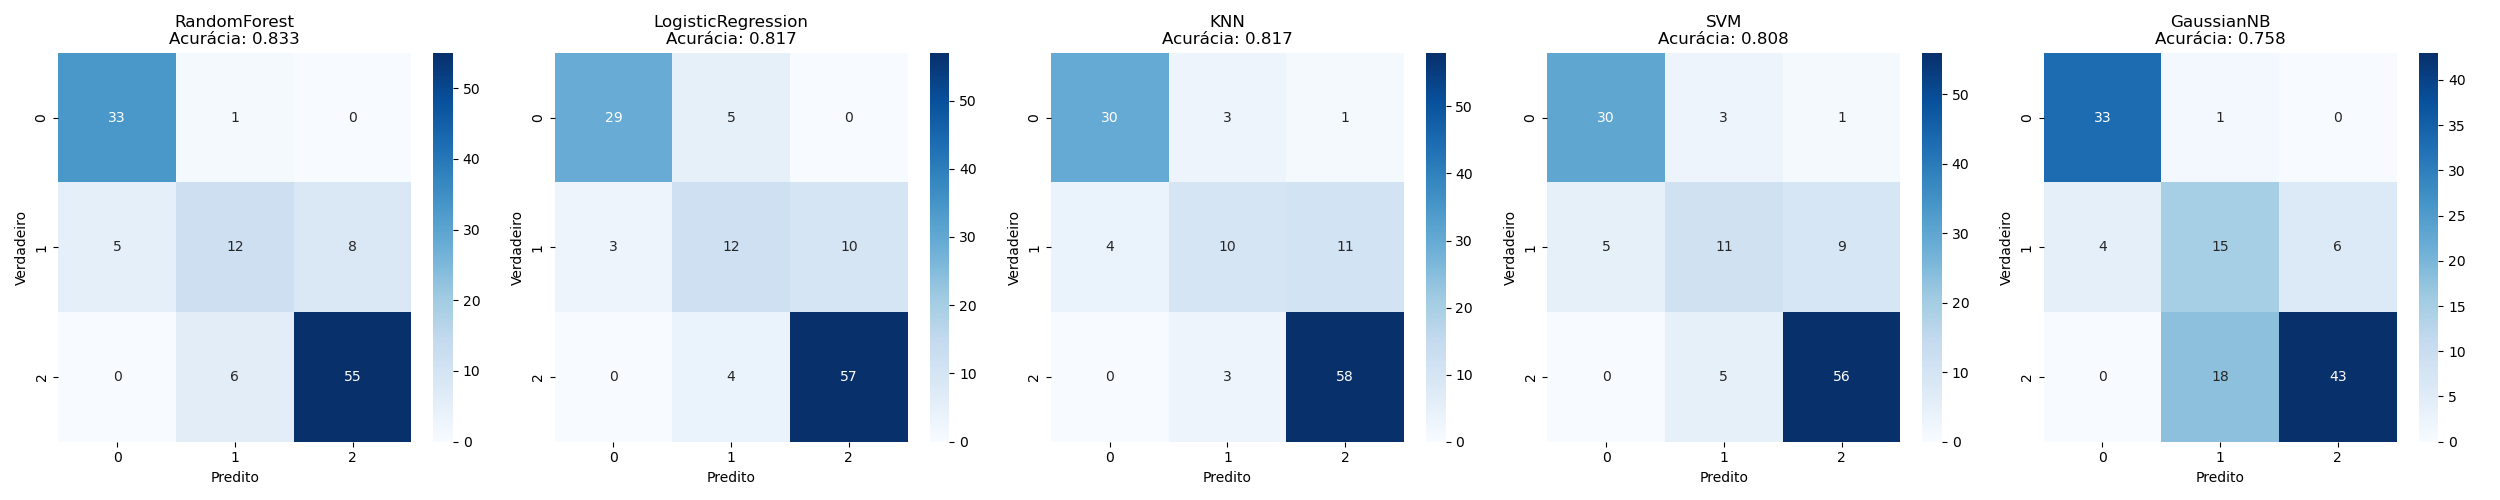
\includegraphics[width=1\textwidth]{Figures/data_2_5years_premier_league_matriz_confusao_Zero.png}
    \caption{Matriz de confusão do \textit{data\_2} considerando o corte temporal de 5 anos, com os valores das variáveis dos times rebaixados zerados.}
    \label{fig:Figura1}
\end{figure}

\begin{figure}[H]
    \centering
    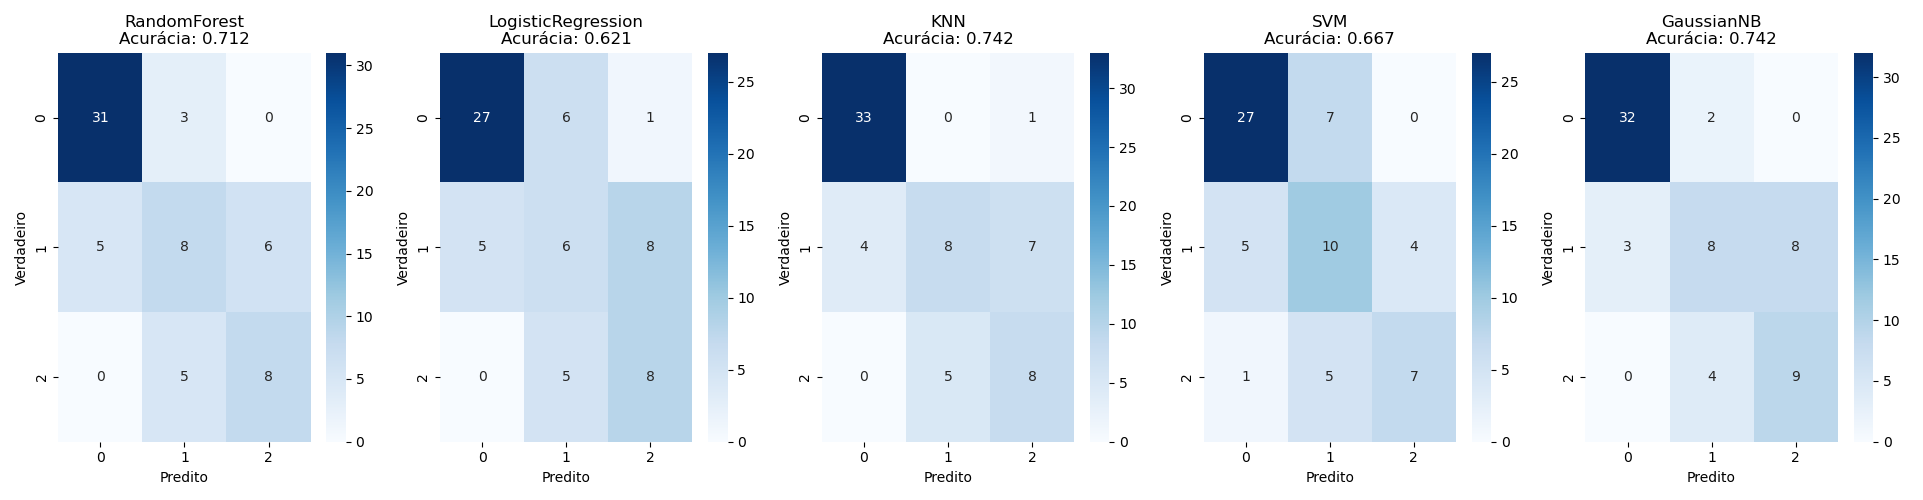
\includegraphics[width=1\textwidth]{Figures/data_2_5years_premier_league_matriz_confusao_exclusao.png}
    \caption{Matriz de confusão do \textit{data\_2} considerando o corte temporal de 5 anos, com os valores das variáveis dos times excluídas.}
    \label{fig:Figura2}
\end{figure}

\begin{figure}[H]
    \centering
    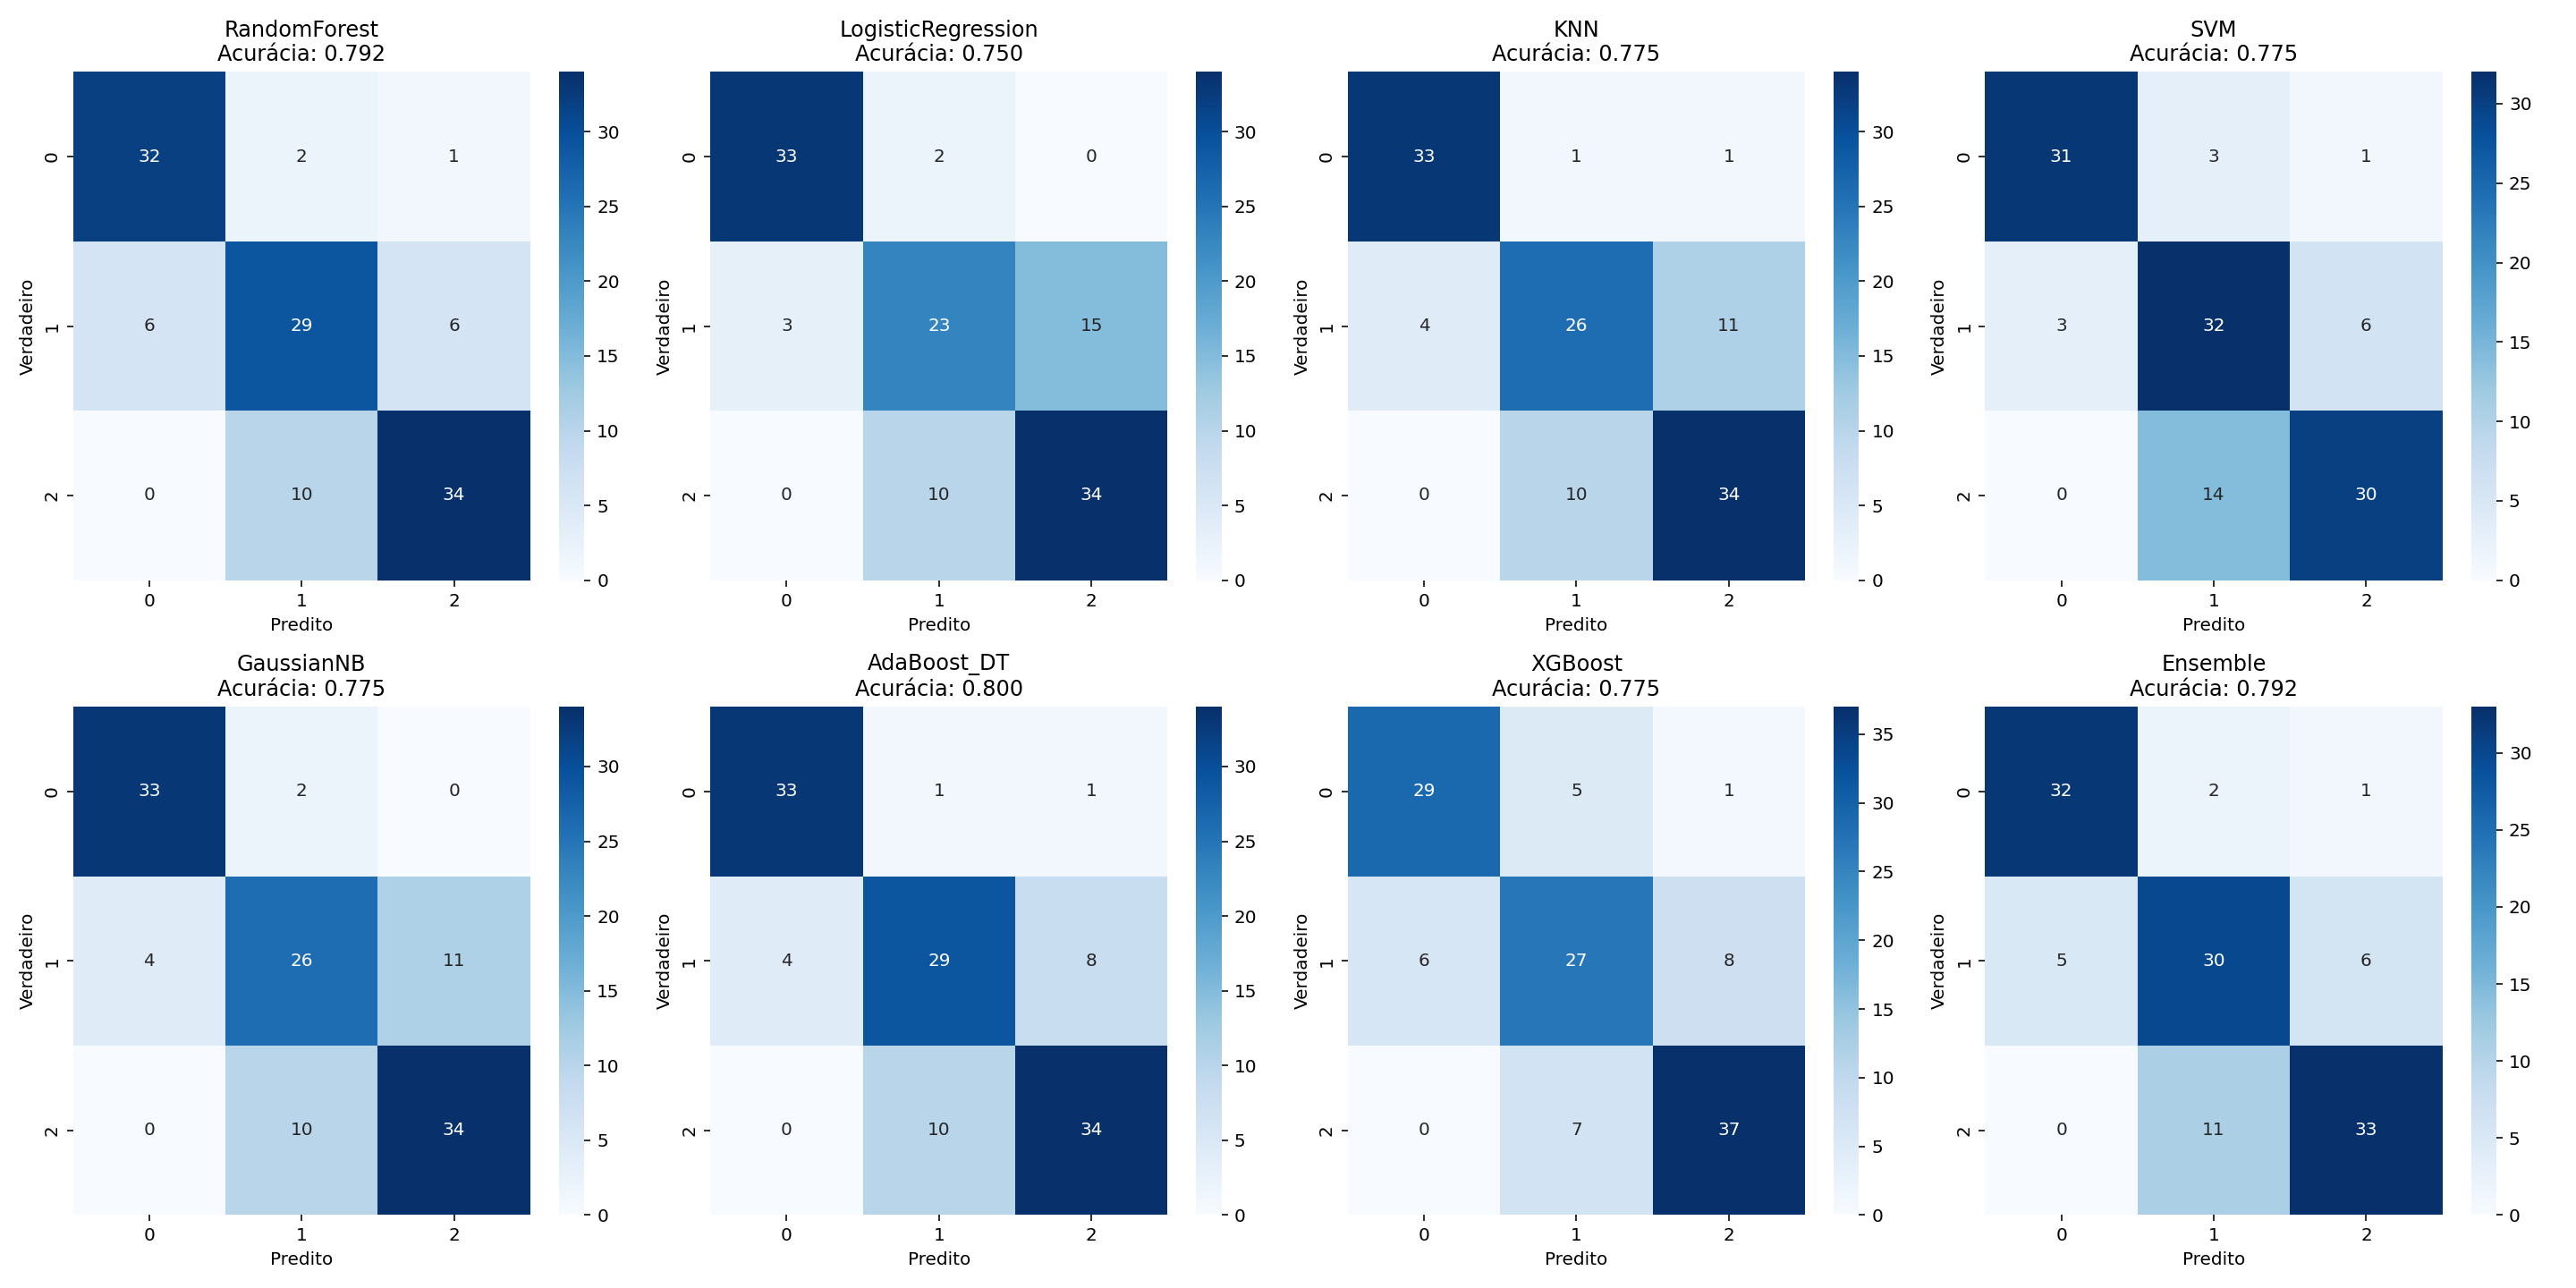
\includegraphics[width=1\textwidth]{Figures/data_2_5years_premier_league_matriz_confusao_repetido.png}
    \caption{Matriz de confusão do \textit{data\_2} considerando o corte temporal de 5 anos, com os valores das variáveis dos times rebaixados repetidos.}
    \label{fig:Figura3}
\end{figure}




\section{Resultados}
Para apresentação dos resultados finais da comparação entre os modelos será realizada uma divisão em subtópicos. Cada subtópio terá como objetivo responder à um dos objetivos específicos enumerados acima.

\subsection{Comparação entre os filtros temporais (1, 3 e 5 anos)}

As acurácias médias dos modelos podem ser observadas nas figuras \ref{fig:Figura4}, \ref{fig:Figura5} e \ref{fig:Figura6}. No segundo conjunto de dados (\texttt{data\_2}), o teste de Friedman para o corte de 5~anos indicou diferença global significativa entre os três \texttt{datasets} ($\chi^{2}=8{,}44$, $p=0{,}015$) na Ligue 1 francesa. O pós-hoc de Nemenyi indicou diferença entre o corte temporal de 1 e 5 anos ($p=0{,}0307$). Em todos os demais casos os testes de Friedman não revelaram diferenças significativas ($p>0{,}05$) entre os cortes temporais de 1, 3 e 5 anos.

\begin{figure}[H]
    \centering
    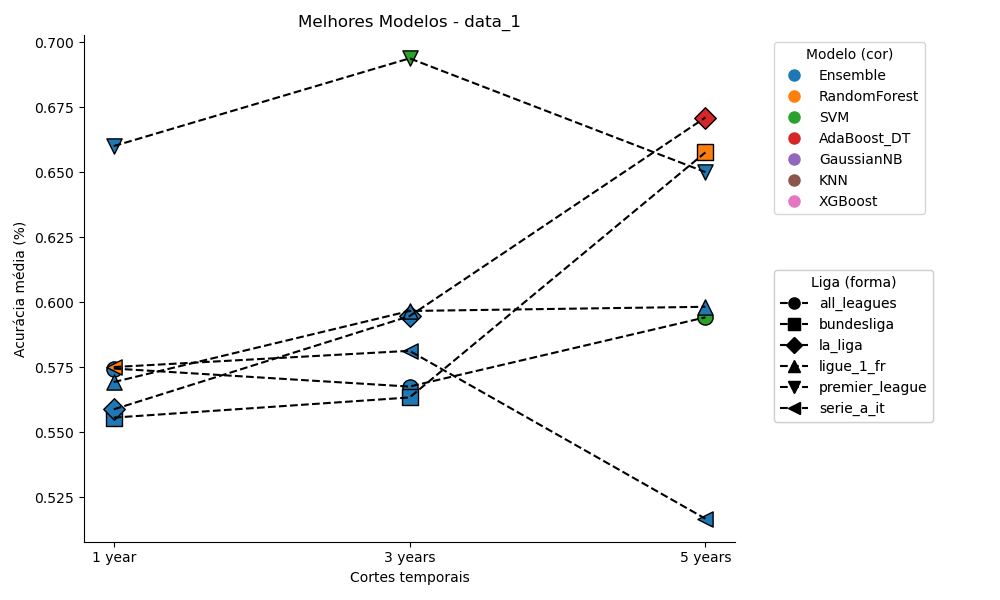
\includegraphics[width=1\textwidth]{Figures/years_data1.png}
    \caption{Acurácia média dos melhores modelos do data 1 nos diferentes cortes temporais}
    \label{fig:Figura4}
\end{figure}

\begin{figure}[H]
    \centering
    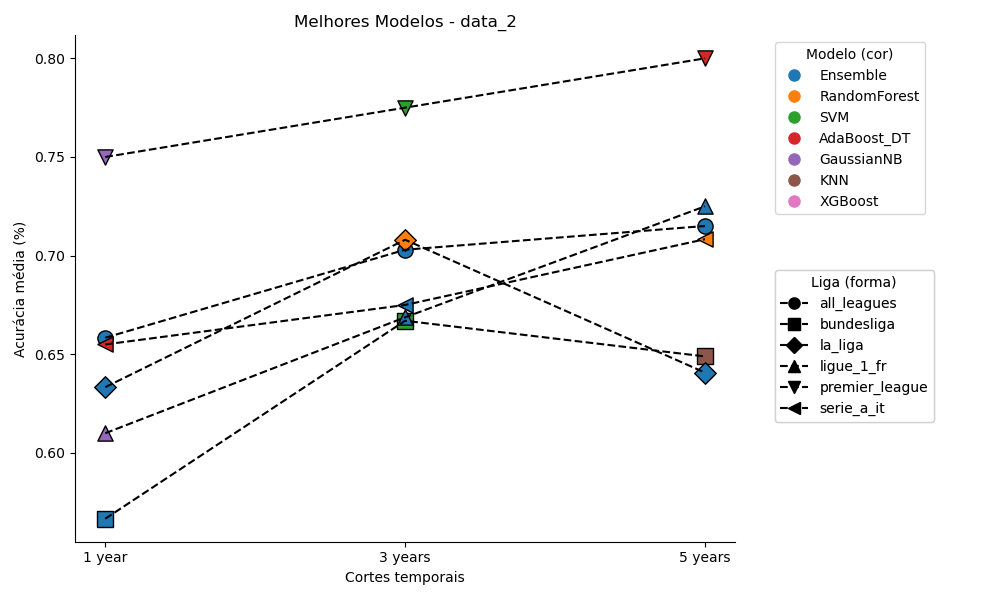
\includegraphics[width=1\textwidth]{Figures/years_data2.png}
    \caption{Acurácia média dos melhores modelos do data 2 nos diferentes cortes temporais}
    \label{fig:Figura5}
\end{figure}

\begin{figure}[H]
    \centering
    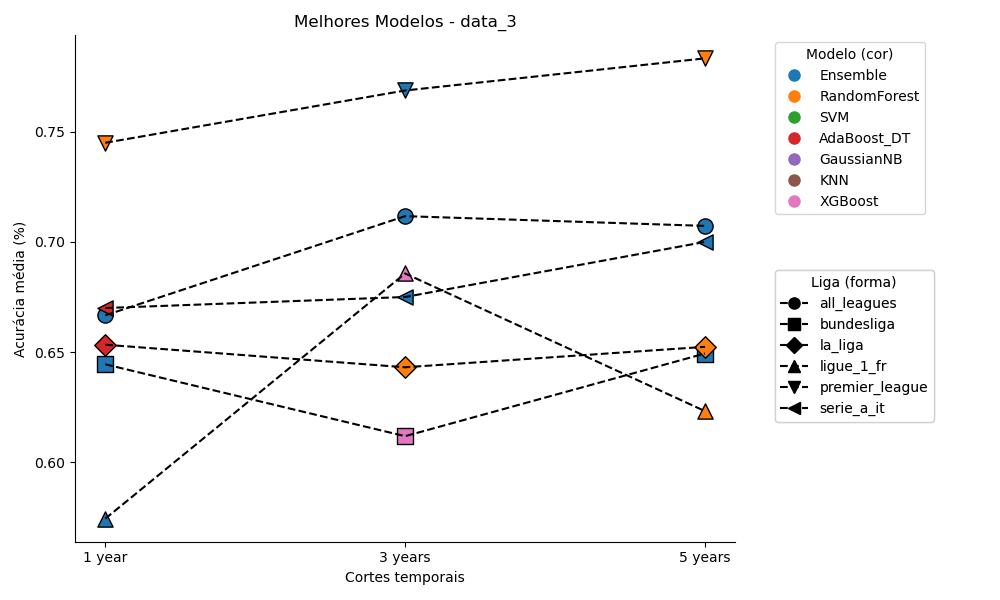
\includegraphics[width=1\textwidth]{Figures/years_data3.png}
    \caption{Acurácia média dos melhores modelos do data 3 nos diferentes cortes temporais}
    \label{fig:Figura6}
\end{figure}


\subsection{Comparação entre os datasets}

 As acurácias médias dos modelos podem ser observadas nas figuras \ref{fig:Figura7}, \ref{fig:Figura8} e \ref{fig:Figura9}. Para todas as ligas combinadas (\textit{all\_leagues}), o teste de Friedman indicou diferença global significativa em 1~ano ($\chi^2=7{,}60$, $p=0{,}022$), 3~anos ($\chi^2=7{,}60$, $p=0{,}022$) e 5~anos ($\chi^2=7{,}60$, $p=0{,}022$). No post hoc, observou-se diferença significativa entre os {\it datasets}~1 e~3 em 1~ano ($p=0{,}031$), entre 1 e~2 em 3~anos ($p=0{,}031$) e novamente entre 1 e~3 em 5~anos ($p=0{,}031$).\\

Na \textit{Bundesliga}, houve diferença global em 3~anos ($\chi^2=7{,}44$, $p=0{,}024$) e o post hoc indicou diferença significativa entre os {\it datasets}~1 e~2 ($p=0{,}031$). Na \textit{La Liga}, o teste de Friedman inidicou diferença no corte de 3~anos ($\chi^2=6{,}00$, $p=0{,}050$), com diferença post hoc entre 1 e~2 ($p=0{,}047$). Na \textit{Premier League}, verificou-se diferença global em 5~anos ($\chi^2=7{,}41$, $p=0{,}025$) e post hoc entre 1 e~2 ($p=0{,}047$). Na \textit{Série A Italiana}, houve diferença global em 1~ano ($\chi^2=8{,}32$, $p=0{,}016$) e 5~anos ($\chi^2=7{,}60$, $p=0{,}022$), com diferenças post hoc entre 1 e~3 em ambas as durações (1~ano: $p=0{,}020$; 5~anos: $p=0{,}031$). Nas demais combinações de liga e duração, não se observaram diferenças significativas ($p>0{,}05$).

 \begin{figure}[H]
    \centering
    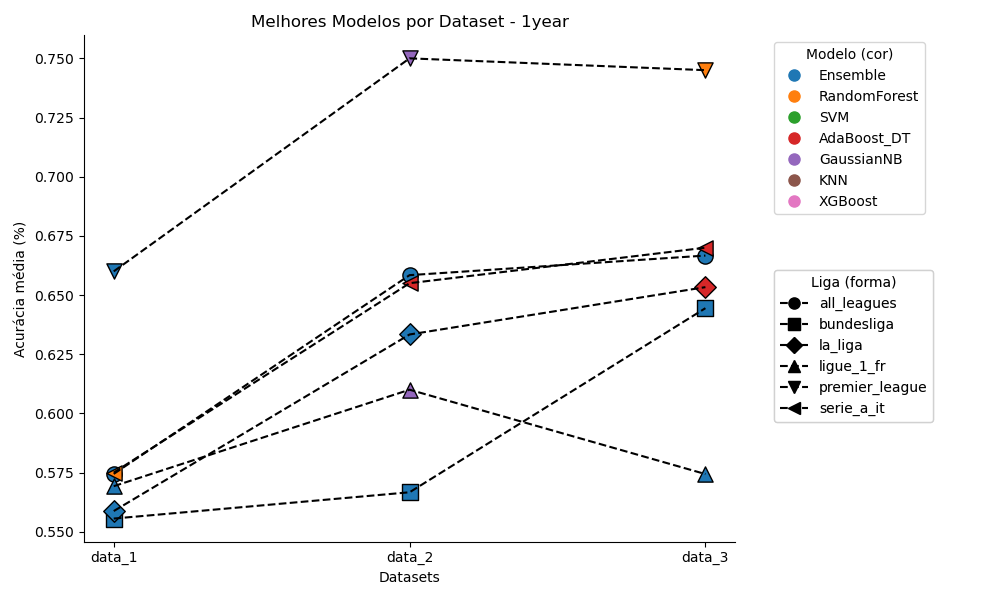
\includegraphics[width=1\textwidth]{Figures/Dataset_1year.png}
    \caption{Acurácia média dos melhores modelos com corte temporal de 1 ano nos diferentes datasets}
    \label{fig:Figura7}
\end{figure}

\begin{figure}[H]
    \centering
    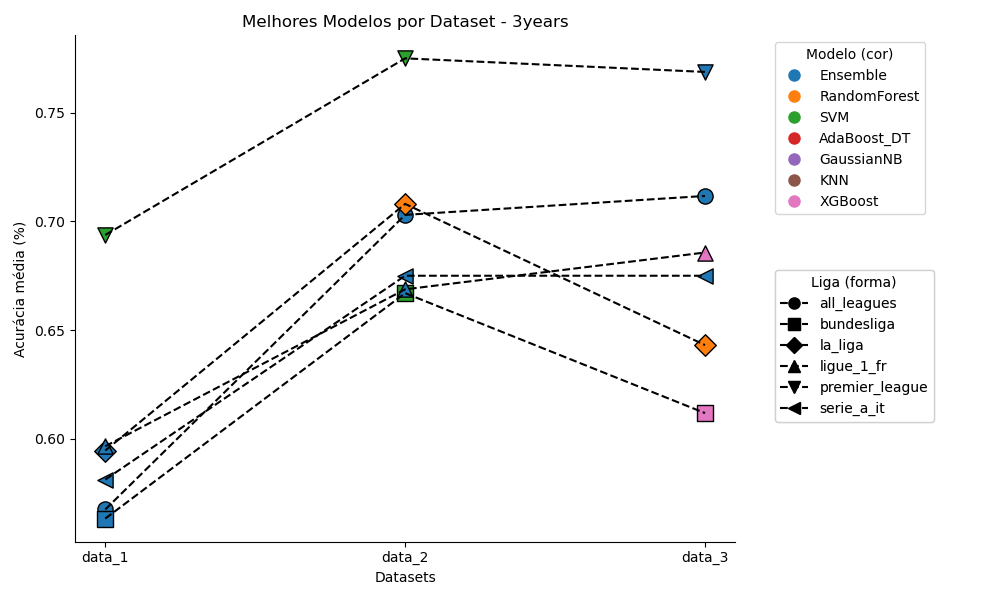
\includegraphics[width=1\textwidth]{Figures/Dataset_3years.png}
    \caption{Acurácia média dos melhores modelos com corte temporal de 3 anos nos diferentes datasets}
    \label{fig:Figura8}
\end{figure}

\begin{figure}[H]
    \centering
    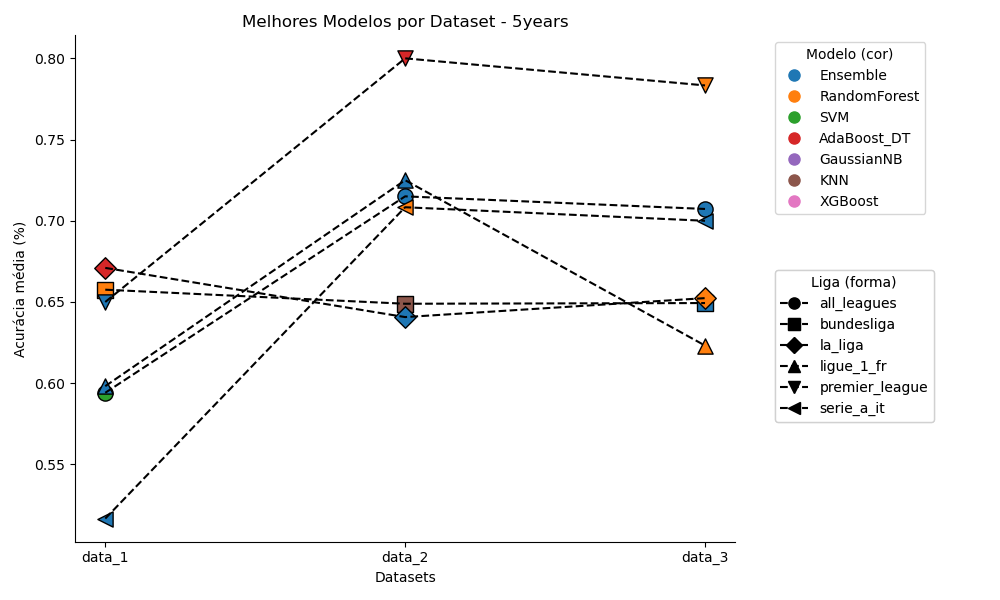
\includegraphics[width=1\textwidth]{Figures/Dataset_5years.png}
    \caption{Acurácia média dos melhores modelos com corte temporal de 5 anos nos diferentes datasets}
    \label{fig:Figura9}
\end{figure}

\subsection{Comparação entre as ligas europeias}

Para o primeiro conjunto de dados, relativo à transferência dos jogadores (\texttt{data\_1}), o teste de Friedman para o corte de 5~anos indicou diferença global significativa entre as ligas analisadas ($\chi^{2}=14{,}71$, $p=0{,}0117$). No pós-hoc de Nemenyi, observou\-se diferenças significativas entre \textit{La Liga} e \textit{Série A Italiana} ($p=0{,}0166$) e entre \textit{Premier League} e \textit{Série A Italiana} ($p=0{,}0284$).

Para o segundo conjunto de dados (\texttt{data\_2}), o teste de Friedman no corte de 1~ano revelou diferença global significativa ($\chi^{2}=13{,}33$, $p=0{,}0204$). No pós-hoc, houve diferença significativa entre \textit{Bundesliga} e \textit{Premier League} ($p=0{,}0218$) e entre \textit{Ligue 1 Francesa} e \textit{Premier League} ($p=0{,}0366$).

Em todos os demais casos — para os cortes de 1 e 3~anos em \texttt{data\_1}, para os cortes de 3 e 5~anos em \texttt{data\_2}, bem como em qualquer duração para os demais conjuntos de dados — os testes de Friedman não revelaram diferenças globais significativas ($p>0{,}05$).




\section{Discussão}
    
Em relação aos modelos de aprendizado de máquina, o ensemble dos melhores modelos foi o que mais se destacou. Isso era esperado levando em conta que eles utiliza a decisão dos três melhores modelos para a tomada de decisão. De forma geral pode-se observar que somente com os dados de transferências (data 1) os modelos apresentaram um desempenho inferior na predição da posição final nas temporadas seguintes. Acredita-se que isso aconteceu por fornecer informações insuficientes para predição. Quando observa-se a utilização do desempenho do time nas temporadas anteriores para predição (data 2) os modelos apresentaram um desempenho um pouco melhor, variando entre as diferentes ligas. Já quando se observa a predição utilizando os dados de desempenho junto com os de transferência (data 3) não foi apresentada uma melhora em relação à somente utilização dos dados de desempenho. 

Já quando se observa o efeito dos cortes temporais nas predições apesar de visualmente parecer que há uma melhora com um corte temporal maior de forma geral não houve diferença significativa entre os cortes de 1, 3 e 5 anos, somente com a excessão da Ligue 1 que apresentou diferença entre a predição no data 2 entre 1 e 5 anos, com melhor predição com o corte temporal maior. Por fim, ao se observar as diferenças entre as predições nas diferentes ligas europeias, pode-se observar claramente que na premier league houve melhores valores de predição o que ficou evidente também nas análises estatísticas.

Acredita-se que este resultado reflete uma maior constância dos times da Premier League, com menores flutuações entre as equipes ao longo dos anos. Ou seja, os time que se destacam acabam tendo esse bom desempenho nos anos seguinte também, o mesmo vale para os times de meio da tabela e aqueles que brigam contra o rebaixamento. Outro estudo também demonstra essa tendência de constância da Premier League, aplicando algoritmos de árvore de decisão para classificar resultados da partida com base na qualidade dos oponentes obteve-se 67,9, 73,9 e 78,4\%  contra oponentes balanceados, mais fortes e mais fracos, respectivamente\cite{bilek2019predicting}.

Entre as limitações do presente estudo, destaca-se o corte temporal de 10 anos devido à exclusão de dados das temporadas em que houve a COVID-19. Além disso, acredita-se que podem ser testadas outras estratégias de gridsearch para melhor otimização do algoritmos. Outra estratégia que pode ser interessante é a realização de seleção de atributos antes do treinamento e avaliação final dos modelos. As maiores dificuldades do presente estudo foram a definição das estratégias de pré-processamento e o balizamento entre custo computacional e estratégias de treinamento e avaliação dos modelos. Por fim, acredita-se que técnicas de aprendizado de máquina para análise esportiva e auxilio na tomada de decisão devem ser empregadas no esporte por demonstrar uma capacidade de predição de fenômenos complexos e descoberta de conhecimento\cite{claudino2019current}.



\section{Conclusão}
O ensemble se destacou para predição da classificação final dos times nas temporadas seguintes. Os diferentes cortes temporais não demonstraram diferença na predição. Em relação à comparação da capacidade de predição entre as ligas europeias, a premier league foi a que demonstrou melhores resultados. Por fim, utilizar dados do desempenho nas temporadas anteriores foi mais efetivo para predição do que a utilização de dados de transferência de mercado. 

\section{Material Suplementar}
Para informações mais detalhadas dos resultados e acessar os scripts desse projeto, acesse o repositório \href{https://github.com/Abel-Chinaglia/Footbal_prediction-Introducao_AM}{Abel-Chinaglia/Footbal\_prediction-Introducao\_AM}

\bibliography{refs}

\end{document}